\section{Stochastic Properties of Random Matrix Factors - 2}

In the second on the series of posts on stochastic properties of factors of random matrices, we look at a yet another simple case involving norm square of elements of QR decomposition of a scaled Rayleigh matrices. More below.

In applications such as Non-Orthogonal Multiple Access (NOMA), the so-called "path loss" plays an important role whereby a channel matrix $\mathbf{H}$ at a receiver is better modelled as a scaled Rayleigh matrix given by $$\mathbf{H} = \frac{1}{\sqrt{L}} \mathbf{G}$$ where $L > 0$ is the path-loss factor and $\mathbf{G}$ the conventional Rayleigh matrix with real and imaginary parts of the elements each $\mathcal{N}(0,1)$.

Let (by QR decomposition) $\mathbf{H} = \mathbf{Q}\mathbf{R}$ where $\mathbf{Q} \in \mathbb{C}^{M\times M}$ is a Unitary matrix, and $\mathbf{R} \in \mathbb{C}^{M\times N}$ is upper triangular. The distribution of the norm square of elements, $|[\mathbf{R}]_{ij}|^2$, of $\mathbf{R}$ is given by $$|[\mathbf{R}]_{ij}|^2 \sim \begin{cases} \Gamma(M+1-i,\frac{2}{L}) & \text{if $i = j$} \\ \Gamma(1,\frac{2}{L}) & \text{if $i < j$} \\ 0 & \text{otherwise,} \end{cases}$$ where $i=1,2,\cdots,M$, $j=1,2,\cdots,N$, and $\Gamma(k,\theta)$ denotes the Gamma distribution with probability density function $$f(x; k,\theta) = \frac{1}{\Gamma(k)\theta^k}x^{(k-1)}e^{-\frac{x}{\theta}}$$ where $\Gamma(k)$ is the complete Gamma function.

The stochastic properties of the diagonal elements of $\mathbf{R}$ are interesting as they can be used to derive insights, amongst others, about mutual information of "layers" (i.e. parallel streams of information, one per row) or the determinant of the covariance matrix of $\mathbf{H}$.

Figure below illustrates the distributions of elements of $\mathbf{R}$ for $M=4, N=2$ computed numerically using MATLAB. Normalized numerical quantities obtained over 100000 trials are plotted in the blue bar graph and the theoretical expectation is plotted in red. Numerical results closely match the theoretical expectation.

\begin{figure}[H]
	\centering
	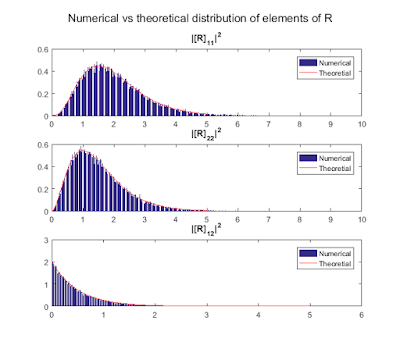
\includegraphics[width=0.5\textwidth,keepaspectratio]{008_001_smf-2.png}
\end{figure}

ARK

\emph{First published: 25th Aug. 2017 on aravindhk-math.blogspot.com}
